\documentclass{article}
\usepackage[margin=1in, paperwidth=8.5in, paperheight=11in]{geometry}
\usepackage{caption}
\usepackage{subcaption}
\usepackage{float}
\usepackage{graphicx}
\usepackage[utf8]{inputenc}
\usepackage{hyperref}

\begin{document}


\subsection{Ready-To-Drive-Sound (RTDS)}
\subsubsection{Description}
%Describe your concept of the RTDS, how is the sound produced, what are the parameters for activating the RTDS, etc.
The Ready to Drive sound is located as a component of the dashboard subsystem, and contains a buzzer (\href{http://cirlw3yrzg4afc1x47lv2k18.wpengine.netdna-cdn.com/wp-content/uploads/2016/12/WT-1205-new.pdf}{Link: Soberton Inc. WT-1205}). The buzzer automatically makes a noise when given power, with the loudness proportional
to the voltage. The last step in the start up sequence will notify the CAN system it is time for the ready
to drive sound. Then the corresponding node on the buzzer will close a relay between TS+, after a 1.2 K$\Omega$
resistor, and the buzzer for two seconds. The resistor limits the voltage over the buzzer to 48V
and the current to 20 mA.
\subsubsection{Wiring, cables, current calculations, connectors}
%Describe wiring, show schematics, describe connectors and cables and show useful data regarding the wiring.
When the shutdown circuit closes and activates the AIRs, the car is in ready to drive mode. As soon as the
car is in this mode, the CAN system will activate the ready to drive sound node to send a positive output
that powers the relay for 2 seconds, thus letting the buzzer sound for 2 seconds. The resistor will be current-limiting and act in the place of a fuse.


\begin{figure}[h]
	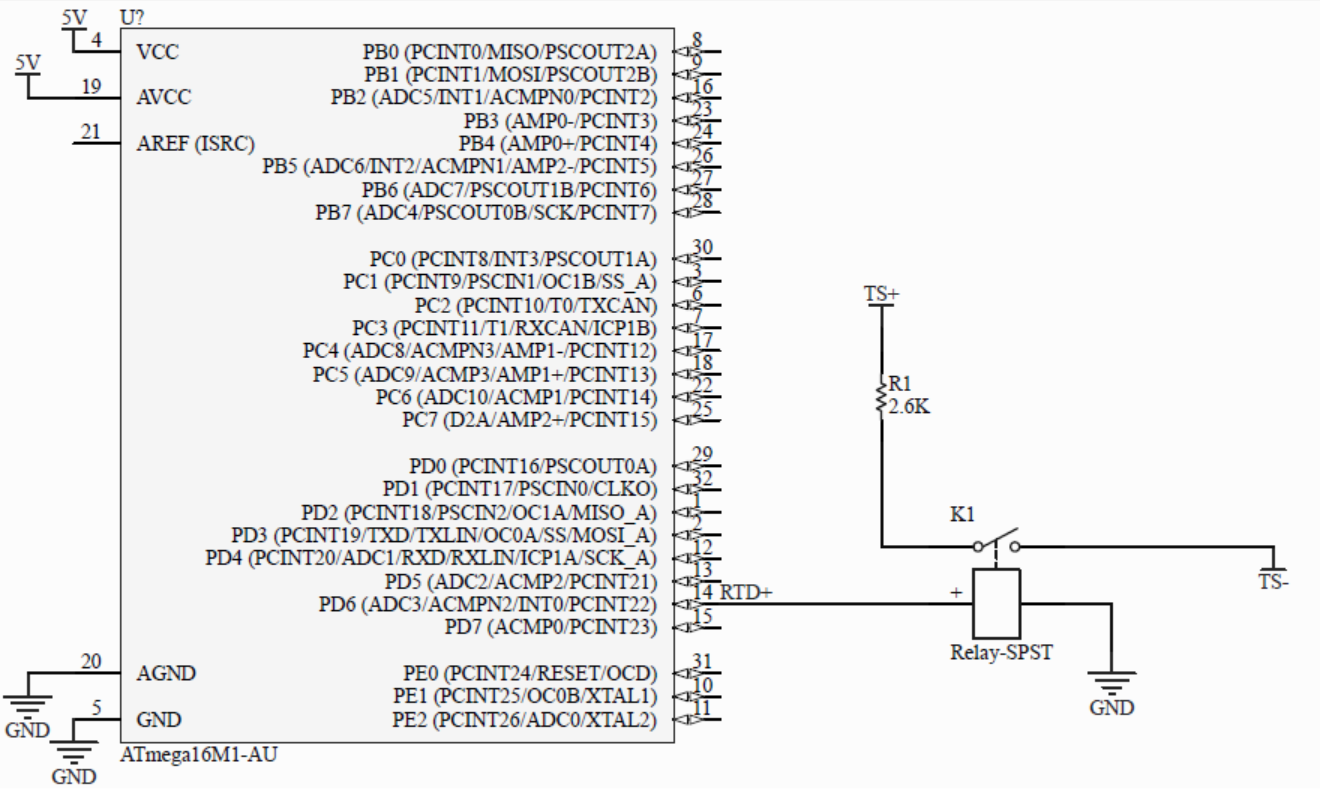
\includegraphics[width=\linewidth]{Schematic}
	\caption{Ready to Drive Sound Schematic as a subsystem of the dashboard's PCB}
\end{figure}
%Begin Equations
	\begin{equation}
		\centering
		V=I*R
	\end{equation}
	\begin{equation}
		\centering
		298-48V=0.021A*R
	\end{equation}
	\begin{equation}
		\centering
		R=1190\Omega
	\end{equation}
%End Equations

%Begin Equations
	\begin{equation}
		\centering
		P=I*V
	\end{equation}
	\begin{equation}
		\centering
		P=0.021A*250V
	\end{equation}
	\begin{equation}
		\centering
		P=5.25W
	\end{equation}
%End Equations
According to these equations, a 1.2K$\Omega$ resistor will function as a current limiting resistor.
\subsubsection{Position in car}
%Provide CAD-renderings showing all relevant parts. Mark the parts in the rendering, if necessary.
The ready to drive sound will be located in the dashboard enclosure shown in Figure !!!!. The buzzer will be mounted
to the exterior and underside of this enclosure. It must be contained outside of the box so that the buzzer is
loud enough and underneath to assist with water proofing of the container
\end{document}
